\begin{frame}{system design}
    \begin{columns}
        \begin{column}{0.5\textwidth}
            \begin{figure}
                \centering
                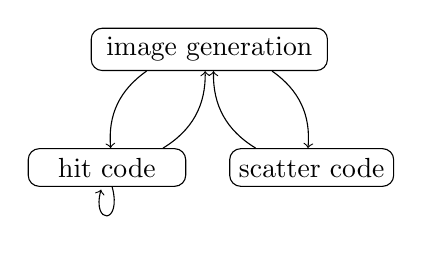
\begin{tikzpicture}[->]
                    \node[draw, rectangle, rounded corners, minimum width=3cm] (A) at (0, 0) {image generation};
                    \node[draw, rectangle, rounded corners, minimum width=2cm] (B) at (-1.3, -1.5) {hit code};
                    \node[draw, rectangle, rounded corners, minimum width=2cm] (C) at (1.3, -1.5) {scatter code};
                    
                    \draw (A) edge[bend right] (B);
                    \draw (B) edge[bend right] (A);

                    \draw (A) edge[bend left] (C);
                    \draw (C) edge[bend left] (A);
                    
                    \path (B) edge [loop below] (B);
                \end{tikzpicture}
                \caption{Ray tracer overview }
            \end{figure}
        \end{column}
        \pause
        \begin{column}{0.5\textwidth}
            \begin{itemize}
                \item Complex enough system to demonstrate the idea in an applied setting.
                \pause 
                \item Distinct components that can be isolated for testing.
                \pause 
                \item Requires high performance to function effectively, making it ideal for assessing performance needs.
            \end{itemize}
        \end{column}
    \end{columns}
\end{frame}